\documentclass[12pt]{article}
\usepackage[letterpaper,margin=0.7in,headheight=15pt,headsep=16pt,footskip=25pt]{geometry}
\usepackage{tikz,array,fancyhdr,lmodern}
\renewcommand{\familydefault}{\sfdefault}
\pagestyle{fancy}\fancyhf{}\renewcommand{\headrulewidth}{0.35pt}
\fancyhead[L]{\small Week 24 / Three random decks encore / Grades 2--5}
\fancyfoot[L]{\scriptsize Bellingham Math Circle / Week 24 / W24-BON-v1}\fancyfoot[R]{\scriptsize\thepage}
\setlength{\parindent}{0pt}\setlength{\parskip}{9pt}
\newcommand{\problem}[2]{\par\textbf{Problem #1:} #2\par}
\newcommand{\deck}[2]{\begin{tikzpicture}[baseline=0]\node at (-0.6,0.4){\textbf{#1}};\foreach \n [count=\i] in {#2}{\draw[rounded corners=2pt] (\i*0.9-0.9,0) rectangle ++(0.7,0.85);\node at (\i*0.9-0.55,0.425){\Large\n};}\end{tikzpicture}}
\newcommand{\lines}[1]{\foreach \y in {1,...,#1}{\par\vspace{20pt}\hrule height 0.3pt\relax}}
\newcommand{\triples}{\begin{tabular}{|p{0.35in}|p{0.35in}|p{0.35in}|p{0.55in}|}\hline A&B&C&Winner\\\hline\rule{0pt}{24pt}&&&\\\hline\rule{0pt}{24pt}&&&\\\hline\rule{0pt}{24pt}&&&\\\hline\rule{0pt}{24pt}&&&\\\hline\rule{0pt}{24pt}&&&\\\hline\rule{0pt}{24pt}&&&\\\hline\rule{0pt}{24pt}&&&\\\hline\rule{0pt}{24pt}&&&\\\hline\rule{0pt}{24pt}&&&\\\hline\end{tabular}}
\newcommand{\totalrows}{\begin{tabular}{|p{0.40in}|p{0.40in}|p{0.48in}|}\hline First&Second&Total\\\hline\rule{0pt}{24pt}&&\\\hline\rule{0pt}{24pt}&&\\\hline\rule{0pt}{24pt}&&\\\hline\rule{0pt}{24pt}&&\\\hline\rule{0pt}{24pt}&&\\\hline\rule{0pt}{24pt}&&\\\hline\rule{0pt}{24pt}&&\\\hline\rule{0pt}{24pt}&&\\\hline\rule{0pt}{24pt}&&\\\hline\end{tabular}}
\begin{document}
Each bag has the three cards shown below. Draw without looking. Put each card back and mix the bag before the next draw. Draws from different bags are separate.

\deck{A}{2,4,9}\hfill\deck{B}{1,6,8}\hfill\deck{C}{3,5,7}

\problem{1}{Draw one card from each bag. The largest card wins. Which bag wins most often? Settle it by finding every possible triple.}
\vspace{8pt}
\triples\hfill\triples\hfill\triples
\vspace{22pt}
\begin{tabular}{|p{1.2in}|p{1.2in}|p{1.2in}|}\hline A wins&B wins&C wins\\\hline\rule{0pt}{33pt}&&\\\hline\end{tabular}
\lines{2}
\newpage
\deck{A}{2,4,9}\hfill\deck{B}{1,6,8}\hfill\deck{C}{3,5,7}
\problem{2}{Draw twice from the same bag, putting the first card back before the second draw. Add the two numbers. Find every possible first-card, second-card pair for each bag and its total.}
\vspace{4pt}
\begin{minipage}[t]{0.31\linewidth}\centering A\par\totalrows\end{minipage}\hfill
\begin{minipage}[t]{0.31\linewidth}\centering B\par\totalrows\end{minipage}\hfill
\begin{minipage}[t]{0.31\linewidth}\centering C\par\totalrows\end{minipage}
\vspace{26pt}
\lines{4}
\newpage
\problem{3}{Each player draws twice from their bag and adds the numbers, as in Problem 2. A higher total earns 2 points; equal totals earn 1 point each. For each pair of bags, which player earns more points on average? Find the wins and ties among every possible four-card draw.}
\vspace{8pt}
\begin{tabular}{|p{1in}|p{1.25in}|p{1.25in}|p{1.25in}|}\hline Bags&First bag wins&Second bag wins&Ties\\\hline\rule{0pt}{42pt} A against B&&&\\\hline\rule{0pt}{42pt} B against C&&&\\\hline\rule{0pt}{42pt} C against A&&&\\\hline\end{tabular}
\vspace{22pt}
\lines{9}
\newpage
\problem{4}{Put label slips A, B, C in a private bag. Your opponent does the same. Secretly draw a label, replace it, and mix your bag. Each player then draws one card from the named deck. Use separate copies if both labels match. The larger card earns 2 points; a tie earns 1 point each.}
\begin{center}
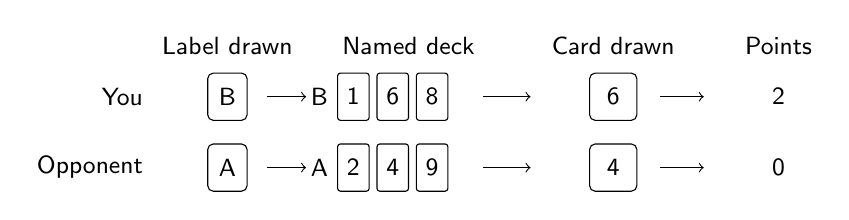
\begin{tikzpicture}[x=1cm,y=1cm,font=\small]
\node at (0.8,1.55){Label drawn};\node at (3.1,1.55){Named deck};\node at (5.7,1.55){Card drawn};\node at (7.8,1.55){Points};
\node[anchor=east] at (-0.15,0.9){You};\node[anchor=east] at (-0.15,0){Opponent};
\foreach \y/\label/\cards/\card/\points in {0.9/B/{1,6,8}/6/2,0/A/{2,4,9}/4/0}{
\draw[rounded corners=2pt] (0.55,\y-0.3) rectangle (1.05,\y+0.3);\node at (0.8,\y){\label};
\draw[->] (1.3,\y)--(1.8,\y);
\node[anchor=east] at (2.2,\y){\label};
\foreach \n [count=\i] in \cards {\draw[rounded corners=1pt] (2.2+\i*0.5-0.5,\y-0.3) rectangle ++(0.4,0.6);\node at (2.2+\i*0.5-0.3,\y){\n};}
\draw[->] (4.05,\y)--(4.65,\y);
\draw[rounded corners=2pt] (5.4,\y-0.3) rectangle (6,\y+0.3);\node at (5.7,\y){\card};
\draw[->] (6.3,\y)--(6.85,\y);\node at (7.8,\y){\points};}
\end{tikzpicture}
\end{center}
Play with the three-slip bag. Then make another nonempty label bag using A, B, C slips. Which bag would you choose before knowing your opponent's bag? Check its average points against an opponent who always chooses A, always B, or always C. Here, the average means points averaged over all equally likely label-slip and card draws.\par
\vspace{6pt}
\begin{tabular}{|p{1.4in}|p{1.2in}|p{1.2in}|p{1.2in}|}\hline My label slips&Against A&Against B&Against C\\\hline\rule{0pt}{40pt}A, B, C&&&\\\hline\rule{0pt}{40pt}&&&\\\hline\rule{0pt}{40pt}&&&\\\hline\end{tabular}
\vspace{12pt}
\problem{5}{Can a label bag earn more than 1 point per round on average against each of A, B, and C? Explain using the possible draws.}
\lines{3}
\end{document}
